\documentclass[border=5mm]{standalone}
\usepackage{tikz}
\usetikzlibrary{calc}
\begin{document}
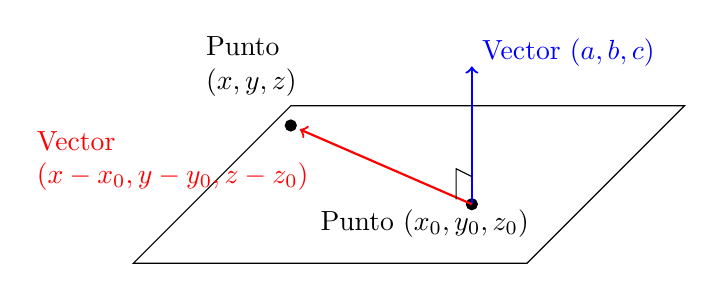
\begin{tikzpicture}
    \draw (0, 0) -- (2, 2) -- (7, 2) -- (5, 0) -- cycle;
    
    \node at (2, 1.75) (b) {};
    \draw [fill] (4.3, 0.75) circle (2pt);
    \draw [fill] (b) circle (2pt);
    \draw [->, color=blue, thick] (4.3, 0.75) -- (4.3, 2.5) node [right, pos=1.1] {Vector $(a, b, c)$};
    
    \draw [->, color=red, thick] (4.3, 0.75) -- ($(4.3, 0.75) !0.95! (b)$);
    
    \draw (4.3, 1.1) -- (4.1, 1.2) -- (4.1, 0.81);
    
    \node at (3.7, 0.5) {Punto $(x_{0}, y_{0}, z_{0})$};
    
    \node [align=left] at (1.5, 2.5) {Punto \\ $(x, y, z)$};

    \node [color=red, align=left] at (0.5, 1.3) {Vector \\ $(x-x_{0}, y-y_{0}, z-z_{0})$};

\end{tikzpicture}
\end{document}